% answers.tex —— 2012 年·安徽卷·文科 · 参考答案与详细解析片段
% 由 tools/generate_projects.py 依来源总账自 2012/2012_数学真题_安徽文_试题.md + 2012/2012_数学真题_安徽文_解析正文.md + 2012/2012_数学真题_安徽文_答案要点.md 生成，勿手改（改源 MD 后重跑）

\begin{answer}
\gksolhead{1}{}

\textbf{题目}：

复数 $z$ 满足 $(z-\mathrm i)\mathrm i=2+\mathrm i$，则 $z=$\mbox{（　　）}

（A）$-1-\mathrm i$；（B）$1-\mathrm i$；（C）$-1+3\mathrm i$；（D）$1-2\mathrm i$。

\Needspace{4\baselineskip}
\textbf{解析}
\Needspace{5\baselineskip}
由 $(z-\mathrm i)\mathrm i=2+\mathrm i$ 得
\nopagebreak[4]
\[z-\mathrm i=\frac{2+\mathrm i}{\mathrm i}=\frac{(2+\mathrm i)(-\mathrm i)}{1}=1-2\mathrm i,\]
故 $z=1-\mathrm i$。选 B。

\gkanswer{答案：B。}

\end{answer}
\begin{answer}
\gksolhead{2}{}

\textbf{题目}：

设集合 $A=\{x\mid-3\leqslant2x-1\leqslant3\}$，集合 $B$ 为函数 $y=\lg(x-1)$ 的定义域，则 $A\cap B=$\mbox{（　　）}

（A）$(1,2)$；（B）$[1,2]$；（C）$[1,2)$；（D）$(1,2]$。

\Needspace{4\baselineskip}
\textbf{解析}
\Needspace{5\baselineskip}
由 $-3\leqslant2x-1\leqslant3$ 得 $-1\leqslant x\leqslant2$，即 $A=[-1,2]$；由 $x-1>0$ 得 $B=(1,+\infty)$。故
\nopagebreak[4]
\[A\cap B=(1,2].\]
选 D。

\gkanswer{答案：D。}

\end{answer}
\begin{answer}
\gksolhead{3}{}

\textbf{题目}：

$\log_29\cdot\log_34=$\mbox{（　　）}

（A）$\dfrac14$；（B）$\dfrac12$；（C）$2$；（D）$4$。

\Needspace{4\baselineskip}
\textbf{解析}
\nopagebreak[4]
\[\log_29\cdot\log_34=\frac{\lg9}{\lg2}\cdot\frac{\lg4}{\lg3}=\frac{2\lg3}{\lg2}\cdot\frac{2\lg2}{\lg3}=4.\]
选 D。

\gkanswer{答案：D。}

\end{answer}
\begin{answer}
\gksolhead{4}{}

\textbf{题目}：

命题“存在实数 $x$，使 $x>1$”的否定是\mbox{（　　）}

（A）对任意实数 $x$，都有 $x>1$；（B）不存在实数 $x$，使 $x\leqslant1$；（C）对任意实数 $x$，都有 $x\leqslant1$；（D）存在实数 $x$，使 $x\leqslant1$。

\Needspace{4\baselineskip}
\textbf{解析}
特称命题的否定是全称命题，“存在 $x$ 使 $x>1$”的否定为“对任意实数 $x$，都有 $x\leqslant1$”。选 C。

\gkanswer{答案：C。}

\end{answer}
\begin{answer}
\gksolhead{5}{}

\textbf{题目}：

公比为 $2$ 的等比数列 $\{a_n\}$ 的各项都是正数，且 $a_3a_{11}=16$，则 $a_5=$\mbox{（　　）}

（A）$1$；（B）$2$；（C）$4$；（D）$8$。

\Needspace{4\baselineskip}
\textbf{解析}
\Needspace{5\baselineskip}
设首项为 $a_1$，则 $a_3a_{11}=a_1^2q^{12}=a_1^2\cdot2^{12}=16$，故 $a_1^2=2^{-8}$，$a_1=2^{-4}$。于是
\nopagebreak[4]
\[a_5=a_1q^4=2^{-4}\cdot2^4=1.\]
选 A。

\gkanswer{答案：A。}

\end{answer}
\begin{answer}
\gksolhead{6}{}

\textbf{题目}：

如图所示，程序框图（算法流程图）的输出结果是\mbox{（　　）}
\nopagebreak[4]
\begin{center}% 2012 年安徽卷文科第 6 题：输出 y 的程序框图。
% 来源 PDF：普通高考/2012/2012安徽文.pdf，第 1 页（印面 715）左栏。
% 流程：开始 → x=1,y=1 → x≤4? 是：x=2x，y=y+1，回到判断；否：输出 y → 结束。
\begin{tikzpicture}[semithick, >=Stealth,
  block/.style={draw, minimum width=3.2cm, minimum height=0.62cm, align=center},
  dec/.style={draw, diamond, aspect=2.6, inner sep=1pt, align=center},
  term/.style={draw, rounded corners=6pt, minimum width=1.5cm, minimum height=0.52cm},
  io/.style={draw, trapezium, trapezium left angle=70, trapezium right angle=110,
             minimum width=2.2cm, minimum height=0.58cm},
  arr/.style={->}]
  \node (start) [term] at (0,6.6) {开始};
  \node (init)  [block] at (0,5.7) {$x=1,\ y=1$};
  \node (dec)   [dec]  at (0,4.35) {$x\leqslant4$?};
  \node (body)  [block] at (3.7,4.35) {$x=2x,\ y=y+1$};
  \node (out)   [io]   at (0,2.95) {输出 $y$};
  \node (end)   [term] at (0,1.95) {结束};
  \draw[arr] (start) -- (init);
  \draw[arr] (init) -- (dec);
  \draw[arr] (dec) -- node[above] {是} (body);
  \draw[arr] (body.north) -- (3.7,5.0) -- (0,5.0);
  \draw[arr] (dec) -- node[right] {否} (out);
  \draw[arr] (out) -- (end);
\end{tikzpicture}
\end{center}
\nopagebreak[4]
（A）$3$；（B）$4$；（C）$5$；（D）$8$。

\Needspace{4\baselineskip}
\textbf{解析}
\Needspace{5\baselineskip}
初始 $x=1$，$y=1$。循环体为 $x=2x$，$y=y+1$，再判断 $x\leqslant4$：
\nopagebreak[4]
\[(x,y)=(2,2)\to(4,3)\to(8,4),\]
当 $x=8$ 时 $x\leqslant4$ 不成立，输出 $y=4$。选 B。

\gkanswer{答案：B。}

\end{answer}
\begin{answer}
\gksolhead{7}{}

\textbf{题目}：

要得到函数 $y=\cos(2x+1)$ 的图象，只要将函数 $y=\cos2x$ 的图象\mbox{（　　）}

（A）向左平移 $1$ 个单位；（B）向右平移 $1$ 个单位；（C）向左平移 $\dfrac12$ 个单位；（D）向右平移 $\dfrac12$ 个单位。

\Needspace{4\baselineskip}
\textbf{解析}
\nopagebreak[4]
\[y=\cos(2x+1)=\cos\left[2\left(x+\frac12\right)\right],\]
故只需将 $y=\cos2x$ 的图象向左平移 $\dfrac12$ 个单位。选 C。

\gkanswer{答案：C。}

\end{answer}
\begin{answer}
\gksolhead{8}{}

\textbf{题目}：

若 $x$，$y$ 满足约束条件 $\begin{cases}x\geqslant0,\\x+2y\geqslant3,\\2x+y\leqslant3,\end{cases}$ 则 $z=x-y$ 的最小值是\mbox{（　　）}

（A）$-3$；（B）$0$；（C）$\dfrac32$；（D）$3$。

\Needspace{4\baselineskip}
\textbf{解析}
\Needspace{5\baselineskip}
由 $x\geqslant0$，$x+2y\geqslant3$，$2x+y\leqslant3$ 得 $0\leqslant x\leqslant1$，且
\nopagebreak[4]
\[\frac{3-x}2\leqslant y\leqslant3-2x.\]
当 $x=0$ 时 $y\in\left[\dfrac32,3\right]$，$z=x-y=-y$ 的最小值为 $-3$（在 $(0,3)$ 处取得）。故 $z_{\min}=-3$。选 A。

\gkanswer{答案：A。}

\end{answer}
\begin{answer}
\gksolhead{9}{}

\textbf{题目}：

若直线 $x-y+1=0$ 与圆 $(x-a)^2+y^2=2$ 有公共点，则实数 $a$ 的取值范围是\mbox{（　　）}

（A）$[-3,-1]$；（B）$[-1,3]$；（C）$[-3,1]$；（D）$(-\infty,-3]\cup[1,+\infty)$。

\Needspace{4\baselineskip}
\textbf{解析}
\Needspace{5\baselineskip}
圆心 $(a,0)$ 到直线 $x-y+1=0$ 的距离不超过半径 $\sqrt2$：
\nopagebreak[4]
\[\frac{|a+1|}{\sqrt2}\leqslant\sqrt2,\]
即 $|a+1|\leqslant2$，解得 $-3\leqslant a\leqslant1$。选 C。

\gkanswer{答案：C。}

\end{answer}
\begin{answer}
\gksolhead{10}{}

\textbf{题目}：

袋中共有 $6$ 个除了颜色外完全相同的球，其中有 $1$ 个红球、$2$ 个白球和 $3$ 个黑球。从袋中任取两球，两球颜色为一白一黑的概率等于\mbox{（　　）}

（A）$\dfrac15$；（B）$\dfrac25$；（C）$\dfrac35$；（D）$\dfrac45$。

\Needspace{4\baselineskip}
\textbf{解析}
\Needspace{5\baselineskip}
从 $6$ 个球中任取两个共有 $\mathrm C_6^2=15$ 种取法，其中一白一黑有 $\mathrm C_2^1\mathrm C_3^1=6$ 种，故概率为
\nopagebreak[4]
\[\frac6{15}=\frac25.\]
选 B。

\gkanswer{答案：B。}

\end{answer}
\begin{answer}
\gksolhead{11}{}

\textbf{题目}：

设向量 $\boldsymbol a=(1,2m)$，$\boldsymbol b=(m+1,1)$，$\boldsymbol c=(2,m)$，若 $(\boldsymbol a+\boldsymbol c)\perp\boldsymbol b$，则 $|\boldsymbol a|=$\gkblank{}。

\Needspace{4\baselineskip}
\textbf{解析}
\Needspace{5\baselineskip}
$\boldsymbol a+\boldsymbol c=(3,3m)$。由 $(\boldsymbol a+\boldsymbol c)\perp\boldsymbol b$ 得
\nopagebreak[4]
\[3(m+1)+3m=0,\]
解得 $m=-\dfrac12$。于是 $|\boldsymbol a|=\sqrt{1+4m^2}=\sqrt{1+1}=\sqrt2$。

\gkanswer{答案：$\sqrt2$。}

\end{answer}
\begin{answer}
\gksolhead{12}{}

\textbf{题目}：

某几何体的三视图如图所示，该几何体的体积是\gkblank{}。
\nopagebreak[4]
\begin{center}% 2012 年安徽卷文科第 12 题：直棱柱的三视图（单位：cm，图中只标数值）。
% 来源 PDF：普通高考/2012/2012安徽文.pdf，第 1 页（印面 715）中栏。
% 正视图 5×4，内部竖线在 x=2；侧视图 4×4；俯视图为直角梯形，上底 5、下底 2、高 4。
\begin{tikzpicture}[scale=0.70, semithick,
  dim/.style={<->, >=Stealth, thin},
  lab/.style={font=\small}]
  % ---------- 正视图 ----------
  \begin{scope}
    \draw (0,0) rectangle (5,4);
    \draw (2,0) -- (2,4);
    \draw[dim] (-0.45,0) -- (-0.45,4);
    \node[left] at (-0.45,2) {4};
    \node[below] at (2.5,-0.45) {正（主）视图};
  \end{scope}
  % ---------- 侧视图 ----------
  \begin{scope}[shift={(7.6,0)}]
    \draw (0,0) rectangle (4,4);
    \node[below] at (2,-0.45) {侧（左）视图};
  \end{scope}
  % ---------- 俯视图 ----------
  \begin{scope}[shift={(1.2,-6.6)}]
    \draw (0,0) -- (2,0) -- (5,4) -- (0,4) -- cycle;
    \draw[dim] (5.45,0) -- (5.45,4);
    \node[right] at (5.45,2) {4};
    \draw[dim] (0,4.4) -- (5,4.4);
    \node[above] at (2.5,4.4) {5};
    \draw[dim] (0,-0.4) -- (2,-0.4);
    \node[below] at (1,-0.4) {2};
    \node[below] at (2.5,-1.05) {俯视图};
  \end{scope}
\end{tikzpicture}
\end{center}
\nopagebreak[4]
\Needspace{4\baselineskip}
\textbf{解析}
\Needspace{5\baselineskip}
由三视图知该几何体是高为 $4$ 的直棱柱，底面是上底 $5$、下底 $2$、高（纵深）$4$ 的直角梯形。底面积
\nopagebreak[4]
\[S=\frac{(5+2)\times4}2=14,\]
\Needspace{5\baselineskip}
故体积
\nopagebreak[4]
\[V=14\times4=56.\]

\gkanswer{答案：$56$。}

\end{answer}
\begin{answer}
\gksolhead{13}{}

\textbf{题目}：

若函数 $f(x)=|2x+a|$ 的单调递增区间是 $[3,+\infty)$，则 $a=$\gkblank{}。

\Needspace{4\baselineskip}
\textbf{解析}
$f(x)=|2x+a|$ 在 $\left[-\dfrac a2,+\infty\right)$ 上单调递增，由已知 $-\dfrac a2=3$，故 $a=-6$。

\gkanswer{答案：$-6$。}

\end{answer}
\begin{answer}
\gksolhead{14}{}

\textbf{题目}：

过抛物线 $y^2=4x$ 的焦点 $F$ 的直线交该抛物线于 $A$，$B$ 两点，若 $|AF|=3$，则 $|BF|=$\gkblank{}。

\Needspace{4\baselineskip}
\textbf{解析}
\Needspace{5\baselineskip}
抛物线 $y^2=4x$ 的 $p=2$。过焦点的弦满足
\nopagebreak[4]
\[\frac1{|AF|}+\frac1{|BF|}=\frac2p=1,\]
故 $\dfrac13+\dfrac1{|BF|}=1$，得 $|BF|=\dfrac32$。

\gkanswer{答案：$\dfrac32$。}

\end{answer}
\begin{answer}
\gksolhead{15}{}

\textbf{题目}：

若四面体 $ABCD$ 的三组对棱分别相等，即 $AB=CD$，$AC=BD$，$AD=BC$，则\gkblank{}。（写出所有正确结论编号）

① 四面体 $ABCD$ 每组对棱相互垂直；

② 四面体 $ABCD$ 每个面的面积相等；

③ 从四面体 $ABCD$ 每个顶点出发的三条棱两两夹角之和大于 $90^\circ$ 而小于 $180^\circ$；

④ 连接四面体 $ABCD$ 每组对棱中点的线段相互垂直平分；

⑤ 从四面体 $ABCD$ 每个顶点出发的三条棱的长可作为一个三角形的三边长。

\Needspace{4\baselineskip}
\textbf{解析}
三组对棱分别相等的四面体，四个面全等。

① 不一定成立（正四面体才每组对棱垂直），错误；

② 四个面全等，面积相等，正确；

③ 每个顶点处的三个面角恰是一个面的三个内角，其和为 $180^\circ$，不是“大于 $90^\circ$ 而小于 $180^\circ$”，错误；

④ 三组对棱中点的连线（双中线）互相垂直平分，正确；

⑤ 从顶点 $A$ 出发的三条棱 $AB$，$AC$，$AD$ 分别等于面 $BCD$ 的三边 $CD$，$BD$，$BC$，故可构成三角形，正确。

故填 ②④⑤。

\gkanswer{答案：②④⑤。}

\end{answer}
\begin{answer}
\gksolhead{16}{}

\textbf{题目}：

设 $\triangle ABC$ 的内角 $A$，$B$，$C$ 所对的边为 $a$，$b$，$c$，且有 $2\sin B\cos A=\sin A\cos C+\cos A\sin C$。

（1） 求角 $A$ 的大小；

（2） 若 $b=2$，$c=1$，$D$ 为 $BC$ 的中点，求 $AD$ 的长。

\Needspace{4\baselineskip}
\textbf{解析}
\Needspace{5\baselineskip}
\textbf{（1）} 由 $2\sin B\cos A=\sin A\cos C+\cos A\sin C=\sin(A+C)=\sin B$，且 $\sin B\neq0$，得
\nopagebreak[4]
\[2\cos A=1,\]
故 $A=\dfrac\pi3$。

\Needspace{5\baselineskip}
\textbf{（2）} 由余弦定理
\nopagebreak[4]
\[a^2=b^2+c^2-2bc\cos A=4+1-2\times2\times1\times\frac12=3.\]
\Needspace{5\baselineskip}
$D$ 为 $BC$ 中点，由中线长公式
\nopagebreak[4]
\[AD^2=\frac{2b^2+2c^2-a^2}4=\frac{8+2-3}4=\frac74,\]
故 $AD=\dfrac{\sqrt7}2$。

\gkanswer{答案（1）：$A=\dfrac\pi3$。}

\gkanswer{答案（2）：$\dfrac{\sqrt7}2$。}

\end{answer}
\begin{answer}
\gksolhead{17}{}

\textbf{题目}：

设定义在 $(0,+\infty)$ 上的函数 $f(x)=ax+\dfrac1{ax}+b$（$a>0$）。

（1） 求 $f(x)$ 的最小值；

（2） 若曲线 $y=f(x)$ 在点 $(1,f(1))$ 处的切线方程为 $y=\dfrac32x$，求 $a$，$b$ 的值。

\Needspace{4\baselineskip}
\textbf{解析}
\Needspace{5\baselineskip}
\textbf{（1）} 由 $a>0$，$x>0$ 得
\nopagebreak[4]
\[ax+\frac1{ax}\geqslant2\sqrt{ax\cdot\frac1{ax}}=2,\]
等号在 $x=\dfrac1a$ 时成立，故 $f(x)$ 的最小值为 $2+b$。

\Needspace{5\baselineskip}
\textbf{（2）} $f'(x)=a-\dfrac1{ax^2}$，故 $f'(1)=a-\dfrac1a$。由切线斜率为 $\dfrac32$ 得
\nopagebreak[4]
\[a-\frac1a=\frac32,\]
\Needspace{5\baselineskip}
即 $2a^2-3a-2=0$，解得 $a=2$（$a>0$）。又 $f(1)=2+\dfrac12+b$ 在切线 $y=\dfrac32x$ 上，故
\nopagebreak[4]
\[\frac52+b=\frac32,\]
得 $b=-1$。

\gkanswer{答案（1）：$2+b$。}

\gkanswer{答案（2）：$a=2$，$b=-1$。}

\end{answer}
\begin{answer}
\gksolhead{18}{}

\textbf{题目}：

若某产品的直径长与标准值的差的绝对值不超过 $1\ \mathrm{mm}$ 时，则视为合格品，否则视为不合格品。在近期一次产品抽样检查中，从某厂生产的此种产品中，随机抽取 $5000$ 件进行检测，结果发现有 $50$ 件不合格品。计算这 $50$ 件不合格品的直径长与标准值的差（单位：$\mathrm{mm}$），将所得数据分组，得到如下频率分布表：

\begin{center}
\begin{tabular}{lll}
\toprule
分组 & 频数 & 频率 \\
\midrule
$[-3,-2)$ &  & $0.10$ \\
$[-2,-1)$ & $8$ &  \\
$(1,2]$ &  & $0.50$ \\
$(2,3]$ & $10$ &  \\
$(3,4]$ &  &  \\
合计 & $50$ & $1.00$ \\
\bottomrule
\end{tabular}
\end{center}

（1） 将上面表格中缺少的数据填在答题卡的相应位置；

（2） 估计该厂生产的此种产品中，不合格品的直径长与标准值的差落在区间 $(1,3]$ 内的概率；

（3） 现对该厂这种产品的某个批次进行检查，结果发现有 $20$ 件不合格品。据此估算这批产品中的合格品的件数。

\Needspace{4\baselineskip}
\textbf{解析}
\textbf{（1）} 由频率之和为 $1$ 及总频数 $50$，补全表格：

\begin{center}
\begin{tabular}{lll}
\toprule
分组 & 频数 & 频率 \\
\midrule
$[-3,-2)$ & $5$ & $0.10$ \\
$[-2,-1)$ & $8$ & $0.16$ \\
$(1,2]$ & $25$ & $0.50$ \\
$(2,3]$ & $10$ & $0.20$ \\
$(3,4]$ & $2$ & $0.04$ \\
合计 & $50$ & $1.00$ \\
\bottomrule
\end{tabular}
\end{center}

\Needspace{5\baselineskip}
\textbf{（2）} 落在 $(1,3]$ 内的频率为
\nopagebreak[4]
\[0.50+0.20=0.70,\]
故概率估计为 $0.70$。

\Needspace{5\baselineskip}
\textbf{（3）} 不合格品的频率为 $\dfrac{50}{5000}=0.01$，故该批产品总数约为
\nopagebreak[4]
\[\frac{20}{0.01}=2000,\]
合格品约为 $2000-20=1980$ 件。

\gkanswer{答案（1）：$[-3,-2)$：$5$、$0.10$；$[-2,-1)$：$8$、$0.16$；$(1,2]$：$25$、$0.50$；$(2,3]$：$10$、$0.20$；$(3,4]$：$2$、$0.04$。}

\gkanswer{答案（2）：$0.70$。}

\gkanswer{答案（3）：$1980$ 件。}

\end{answer}
\begin{answer}
\gksolhead{19}{}

\textbf{题目}：

如图，长方体 $ABCD-A_1B_1C_1D_1$ 中，底面 $A_1B_1C_1D_1$ 是正方形，$O$ 是 $BD$ 的中点，$E$ 是棱 $AA_1$ 上任意一点。

（1） 证明：$BD\perp EC_1$；

（2） 如果 $AB=2$，$AE=\sqrt2$，$OE\perp EC_1$，求 $AA_1$ 的长。
\nopagebreak[4]
\begin{center}% 2012 年安徽卷文科第 19 题：长方体 ABCD-A1B1C1D1，O 为 BD 中点，E 在 AA1 上。
% 来源 PDF：普通高考/2012/2012安徽文.pdf，第 2 页（印面 716）第 1 栏。
% 斜二测投影：screen(x,y,z) = (x + 0.5y, z + 0.35y)，底面边长 2、高 3√2 ≈ 4.24 量纲。
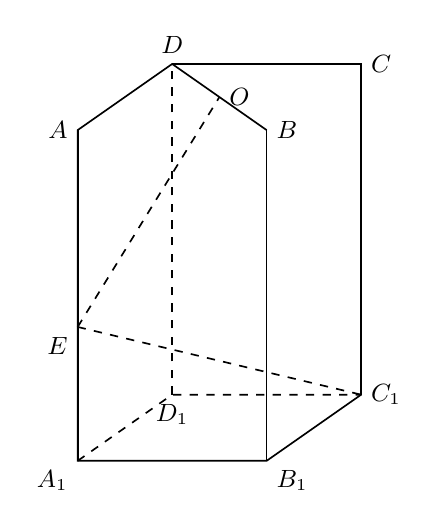
\begin{tikzpicture}[semithick, font=\small]
  % 顶点（x 向右、y 向里、z 向上）
  \coordinate (A1) at (0,0);
  \coordinate (B1) at (2.4,0);
  \coordinate (C1) at (3.6,0.84);
  \coordinate (D1) at (1.2,0.84);
  \coordinate (A)  at (0,4.2);
  \coordinate (B)  at (2.4,4.2);
  \coordinate (C)  at (3.6,5.04);
  \coordinate (D)  at (1.2,5.04);
  \coordinate (O)  at (1.8,4.62);
  \coordinate (E)  at (0,1.7);
  % 实线
  \draw (A1) -- (B1) -- (C1) -- (C) -- (D) -- (A) -- cycle;
  \draw (A1) -- (A);
  \draw (B1) -- (B);
  \draw (C1) -- (C);
  \draw (B) -- (D);
  % 虚线
  \draw[dashed] (A1) -- (D1) -- (C1);
  \draw[dashed] (D1) -- (D);
  \draw[dashed] (E) -- (C1);
  \draw[dashed] (E) -- (O);
  % 标注
  \node[below left] at (A1) {$A_1$};
  \node[below right] at (B1) {$B_1$};
  \node[right] at (C1) {$C_1$};
  \node[below] at (D1) {$D_1$};
  \node[left] at (A) {$A$};
  \node[right] at (B) {$B$};
  \node[right] at (C) {$C$};
  \node[above] at (D) {$D$};
  \node[below left] at (E) {$E$};
  \node[right] at (O) {$O$};
\end{tikzpicture}
\end{center}
\nopagebreak[4]
\Needspace{4\baselineskip}
\textbf{解析}
\Needspace{5\baselineskip}
设底面正方形边长为 $2$，高 $AA_1=h$，取坐标
\nopagebreak[4]
\[A_1(0,0,0),\ B_1(2,0,0),\ C_1(2,2,0),\ D_1(0,2,0),\]
\nopagebreak[4]
\[A(0,0,h),\ B(2,0,h),\ C(2,2,h),\ D(0,2,h).\]
则 $O$ 为 $BD$ 的中点，$O(1,1,h)$；设 $E(0,0,e)$，$0\leqslant e\leqslant h$。

\Needspace{5\baselineskip}
\textbf{（1）} $\overrightarrow{BD}=(-2,2,0)$，$\overrightarrow{EC_1}=(2,2,-e)$，故
\nopagebreak[4]
\[\overrightarrow{BD}\cdot\overrightarrow{EC_1}=-4+4+0=0,\]
即 $BD\perp EC_1$。

\Needspace{5\baselineskip}
\textbf{（2）} $\overrightarrow{OE}=(-1,-1,e-h)$，$\overrightarrow{EC_1}=(2,2,-e)$。由 $OE\perp EC_1$ 得
\nopagebreak[4]
\[-2-2-e(h-e)=0,\]
\Needspace{5\baselineskip}
即 $e(h-e)=4$。又 $AE=e=\sqrt2$，故
\nopagebreak[4]
\[\sqrt2\,(h-\sqrt2)=4,\]
解得 $h=3\sqrt2$，即 $AA_1=3\sqrt2$。

\gkanswer{答案（1）：证明见解析。}

\gkanswer{答案（2）：$3\sqrt2$。}

\end{answer}
\begin{answer}
\gksolhead{20}{}

\textbf{题目}：

如图，$F_1$，$F_2$ 分别是椭圆 $C:\dfrac{x^2}{a^2}+\dfrac{y^2}{b^2}=1$（$a>b>0$）的左、右焦点，$A$ 是椭圆 $C$ 的顶点，$B$ 是直线 $AF_2$ 与椭圆 $C$ 的另一个交点，$\angle F_1AF_2=60^\circ$。

（1） 求椭圆 $C$ 的离心率；

（2） 已知 $\triangle AF_1B$ 面积为 $40\sqrt3$，求 $a$，$b$ 的值。
\nopagebreak[4]
\begin{center}% 2012 年安徽卷文科第 20 题：椭圆两焦点 F1、F2，A 为顶点，B 为直线 AF2 与椭圆的另一交点。
% 来源 PDF：普通高考/2012/2012安徽文.pdf，第 2 页（印面 716）第 2 栏。
% 按 e=1/2 取 a=10、b=5√3≈8.66、c=5，B=(8,-3√3) 的实际比例作图。
\begin{tikzpicture}[scale=0.34, semithick, >=Stealth, font=\small]
  \draw (0,0) ellipse (10 and 8.66);
  \draw[->] (-11.5,0) -- (11.5,0) node[right] {$x$};
  \draw[->] (0,-9.6) -- (0,9.6) node[above] {$y$};
  \coordinate (A) at (0,8.66);
  \coordinate (F1) at (-5,0);
  \coordinate (F2) at (5,0);
  \coordinate (B) at (8,-5.196);
  \draw (A) -- (F1);
  \draw (A) -- (B);
  \draw (F1) -- (B);
  \fill (F1) circle (2.2pt);
  \fill (F2) circle (2.2pt);
  \node[above right] at (A) {$A$};
  \node[below left] at (F1) {$F_1$};
  \node[below right] at (F2) {$F_2$};
  \node[below right] at (B) {$B$};
  \node[below right] at (0,-0.6) {$O$};
\end{tikzpicture}
\end{center}
\nopagebreak[4]
\Needspace{4\baselineskip}
\textbf{解析}
\Needspace{5\baselineskip}
\textbf{（1）} 由 $|AF_1|=|AF_2|=a$，$|F_1F_2|=2c$，$\angle F_1AF_2=60^\circ$ 得
\nopagebreak[4]
\[4c^2=a^2+a^2-2a^2\cos60^\circ=a^2,\]
故 $e=\dfrac ca=\dfrac12$。

\Needspace{5\baselineskip}
\textbf{（2）} 由 $e=\dfrac12$ 得 $a=2c$，$b=\sqrt3c$。取 $A(0,\sqrt3c)$，$F_2(c,0)$，直线 $AF_2$ 的方程为 $y=\sqrt3(c-x)$。代入椭圆
\nopagebreak[4]
\[\frac{x^2}{4c^2}+\frac{y^2}{3c^2}=1\]
得 $x^2+4(c-x)^2=4c^2$，即 $5x^2-8cx=0$，故 $B\left(\dfrac{8c}5,-\dfrac{3\sqrt3c}5\right)$。

\Needspace{5\baselineskip}
于是
\nopagebreak[4]
\[|AB|=\sqrt{\left(\frac{8c}5\right)^2+\left(\frac{8\sqrt3c}5\right)^2}=\frac{16c}5,\]
\Needspace{5\baselineskip}
点 $F_1(-c,0)$ 到直线 $AF_2$：$\sqrt3x+y-\sqrt3c=0$ 的距离为 $\dfrac{|-\sqrt3c-\sqrt3c|}2=\sqrt3c$。故
\nopagebreak[4]
\[S_{\triangle AF_1B}=\frac12\cdot\frac{16c}5\cdot\sqrt3c=\frac{8\sqrt3c^2}5=40\sqrt3,\]
\Needspace{5\baselineskip}
解得 $c=5$，从而
\nopagebreak[4]
\[a=10,\qquad b=5\sqrt3.\]

\gkanswer{答案（1）：$\dfrac12$。}

\gkanswer{答案（2）：$a=10$，$b=5\sqrt3$。}

\end{answer}
\begin{answer}
\gksolhead{21}{}

\textbf{题目}：

设函数 $f(x)=\dfrac x2+\sin x$ 的所有正的极小值点从小到大排成的数列为 $\{x_n\}$。

（1） 求数列 $\{x_n\}$ 的通项公式；

（2） 设 $\{x_n\}$ 的前 $n$ 项和为 $S_n$，求 $\sin S_n$。

\Needspace{4\baselineskip}
\textbf{解析}
\Needspace{5\baselineskip}
\textbf{（1）} $f'(x)=\dfrac12+\cos x$，令 $f'(x)=0$ 得 $x=2k\pi\pm\dfrac{2\pi}3$。又 $f''(x)=-\sin x$，在 $x=2k\pi-\dfrac{2\pi}3$ 处 $f''=\dfrac{\sqrt3}2>0$，为极小值点；在 $x=2k\pi+\dfrac{2\pi}3$ 处为极大值点。由 $x>0$ 得 $k\geqslant1$，故
\nopagebreak[4]
\[x_n=2n\pi-\frac{2\pi}3\quad(n\in\mathbf N^*).\]

\Needspace{5\baselineskip}
\textbf{（2）}
\nopagebreak[4]
\[S_n=\sum_{k=1}^n\left(2k\pi-\frac{2\pi}3\right)=\pi n(n+1)-\frac{2n\pi}3=\frac{\pi n(3n+1)}3.\]
\Needspace{5\baselineskip}
于是
\nopagebreak[4]
\[\sin S_n=\sin\left(n^2\pi+\frac{n\pi}3\right)=(-1)^{n^2}\sin\frac{n\pi}3=(-1)^n\sin\frac{n\pi}3.\]

\gkanswer{答案（1）：$x_n=2n\pi-\dfrac{2\pi}3$（$n\in\mathbf N^*$）。}

\gkanswer{答案（2）：$\sin S_n=(-1)^n\sin\dfrac{n\pi}3$。}

\end{answer}